% CS615 Aspects of System Administration
% Author: Jan Schaumann <jschauma@netmeister.org>
% $Id: slides.tex,v 1.6 2006/03/07 13:55:55 jschauma Exp $

\documentclass[xga]{xdvislides}
\usepackage[landscape]{geometry}
\usepackage{graphics}
\usepackage{graphicx}
\usepackage{colordvi}

\begin{document}
\setfontphv

%%% Headers and footers
\lhead{\slidetitle}                               % default:\lhead{\slidetitle}
\chead{CS615 - Aspects of System Administration}% default:\chead{\relax}
\rhead{Slide \thepage}                       % default:\rhead{\sectiontitle}
\lfoot{\Gray{Development Practices / Backup and Disaster Recovery}}% default:\lfoot{\slideauthor}
\cfoot{\relax}                               % default:\cfoot{\relax}
\rfoot{\Gray{\today}}

\newcommand{\smallish}{\fontsize{15}{20}\selectfont}

\vspace*{\fill}
\begin{center}
	\Hugesize
		CS615 - Aspects of System Administration\\ [1em]
		Development Practices \\ [1em]
		Backup and Disaster Recovery \\ [1em]
	\hspace*{5mm}\blueline\\ [1em]
	\Normalsize
		Department of Computer Science\\
		Stevens Institute of Technology\\
		Jan Schaumann\\
		\verb+jschauma@stevens-tech.edu+
		\verb+http://www.cs.stevens-tech.edu/~jschauma/615A/+
\end{center}
\vspace*{\fill}

\subsection{Midterm Course Survey}
\vspace*{\fill}
{\tt https://www.cs.stevens.edu/\~{}jschauma/cgi-bin/midterm.cgi}
\vspace*{\fill}


\subsection{HW3 Demo / Recap}
\begin{verbatim}
$ ssh linux-lab.cs.stevens.edu
$ export DIR="/home/jschauma/public_html/615/ifcfg-data"
$ for os in fedora freebsd linux-lab netbsd omnios; do
        for flag in i m n; do
                cat ${DIR}/${os} | ifcfg-data -${flag}
        done
done
$
\end{verbatim}

\subsection{User Interface}
\\
\vspace*{\fill}
\begin{center}
	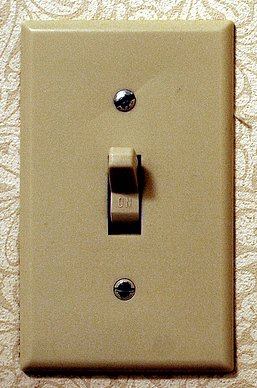
\includegraphics[scale=3]{pics/switch.eps}
\end{center}
\vspace*{\fill}


\subsection{Unix Philosophy}
\\
\Huge
\begin{center}
	Write programs that do one thing and do it well.\\
	\vspace{.5in}
	Write programs to work together. \\
	\vspace{.5in}
	Write programs to handle text streams, because that is a universal interface.
\end{center}
\Normalsize

\subsection{Know your languages / eco-system}
Some advice transcends language: \\

\small
\begin{verbatim}
$ echo import this | python
The Zen of Python, by Tim Peters

Beautiful is better than ugly.
Explicit is better than implicit.
Simple is better than complex.
Complex is better than complicated.
Flat is better than nested.
Sparse is better than dense.
Readability counts.
Special cases aren't special enough to break the rules.
Although practicality beats purity.
Errors should never pass silently.
Unless explicitly silenced.
In the face of ambiguity, refuse the temptation to guess.
There should be one-- and preferably only one --obvious way to do it.
Although that way may not be obvious at first unless you're Dutch.
Now is better than never.
Although never is often better than *right* now.
If the implementation is hard to explain, it's a bad idea.
If the implementation is easy to explain, it may be a good idea.
Namespaces are one honking great idea -- let's do more of those!
\end{verbatim}
\Normalsize


\subsection{POLA}
Principle of Least Astonishment
\\
\vspace*{\fill}
\begin{center}
	
\includegraphics[scale=0.7]{pics/kinder-surprise.eps}
\end{center}
\vspace*{\fill}

\subsection{Know your Users}
Who do we automate things for?
\begin{itemize}
	\item ourselves
	\item our peers
	\item our "users"
	\item anybody else
\end{itemize}

\subsection{Avoid the Quick Fix}
\\
\Huge
\begin{center}
	There's nothing as permanent as a temporary solution.
\end{center}
\Normalsize

\subsection{Take a good look in the mirror!}
\\
\vspace*{\fill}
\begin{center}
	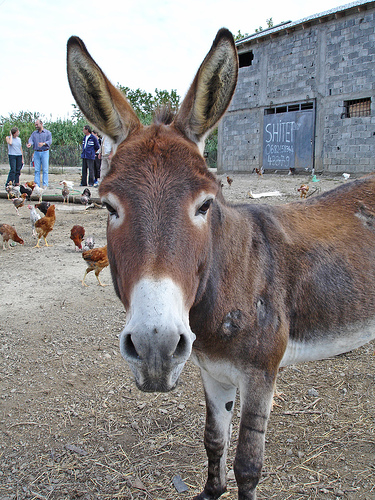
\includegraphics[scale=0.65]{pics/donkey.eps} \\
	\small
	Looks like {\em you} are the ass.
\end{center}
\vspace*{\fill}

\subsection{Learn to write a detailed bug report}
Pre-requisite:
\begin{itemize}
	\item RTFM
	\item Internet Search
	\item Know Your Community
\end{itemize}

\subsection{Learn to write a detailed bug report}
Pre-requisite: Do your homework. \\

Required:
\begin{itemize}
	\item Description Of Problem
	\item Steps To Reproduce
	\item Expected Results
	\item Actual Results
\end{itemize}

\subsection{Learn to write a detailed bug report}
Pre-requisite: Do your homework. \\

Required:
\begin{itemize}
	\item Description Of Problem
	\item Steps To Reproduce
	\item Expected Results
	\item Actual Results
\end{itemize}
\vspace{.125in}

Optional / recommended:
\begin{itemize}
	\item Screenshots / copy and paste terminal I/O
	\item Suggested Remediation
	\item Code Patch
\end{itemize}

\subsection{Avoid the Project That Was Never Finished}
\\
\Huge
\begin{center}
	Don't let the Perfect be the enemy of the Good.
\end{center}
\Normalsize

\subsection{Avoid Feature Creep}
\vspace*{\fill}
\begin{center}
	
\includegraphics[scale=1.0]{pics/feeping.eps} \\
	\small
	\verb+http://www.feepingcreatures.com+
\end{center}
\vspace*{\fill}

\subsection{Release Early, Release Often}
\\
\Huge
\begin{center}
	``More users find more bugs.'' \\
	\addvspace{.2in}
	\small F. Brooks, ``The Mythical Man Month''
\end{center}
\Normalsize

\subsection{Increase the Bus Factor}
\vspace*{\fill}
\begin{center}
	\includegraphics[scale=0.85]{pics/bert-ernie.eps} \\
	\small
	``Just friends.''
\end{center}
\vspace*{\fill}

\subsection{Fix Broken Windows}
\vspace*{\fill}
\begin{center}
	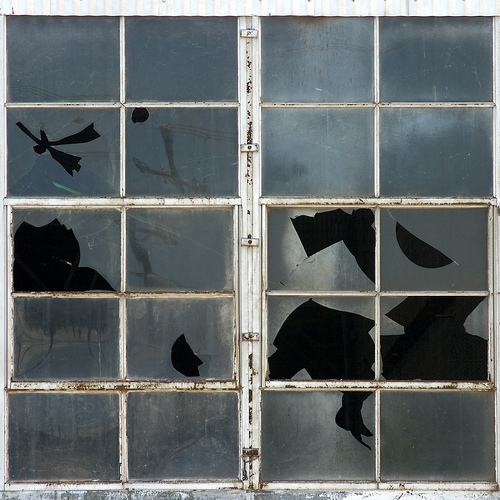
\includegraphics[scale=0.6]{pics/broken-windows.eps}
\end{center}
\vspace*{\fill}

\subsection{Program Maintenance}
\\
\Huge
\begin{center}
	``... is an entropy-increasing process, and even its most skillful
	execution only delays the subsidence of the system into unfixable
	obsolescence.'' \\
	\addvspace{.2in}
	\small F. Brooks, ``The Mythical Man Month''
\end{center}
\Normalsize

\subsection{Toss it!}
\vspace*{\fill}
\begin{center}
	
\includegraphics[scale=3]{pics/waste.eps}
\end{center}
\vspace*{\fill}

\newpage
\vspace*{\fill}
\begin{center}
    \Hugesize
        Hooray! \\ [1em]
    \hspace*{5mm}
    \blueline\\
    \hspace*{5mm}\\
        5 Minute Break
\end{center}
\vspace*{\fill}

\subsection{And now for something completely different...}
\begin{itemize}
	\item backup vs. restore
\end{itemize}

\subsection{And now for something completely different...}
\begin{itemize}
	\item backup vs. restore
	\item backup devices and media
\end{itemize}
\vspace*{\fill}
\begin{center}
	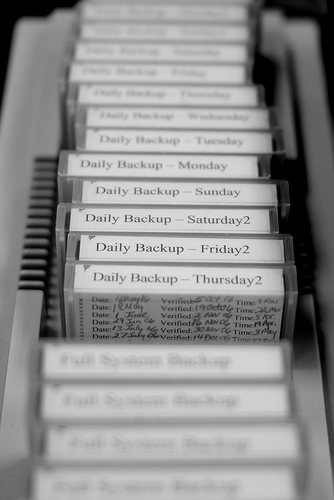
\includegraphics[scale=2.0]{pics/daily-tapes.eps}
\end{center}
\vspace*{\fill}

\subsection{And now for something completely different...}
\begin{itemize}
	\item backup vs. restore
	\item backup devices and media
\end{itemize}
\vspace*{\fill}
\begin{center}
	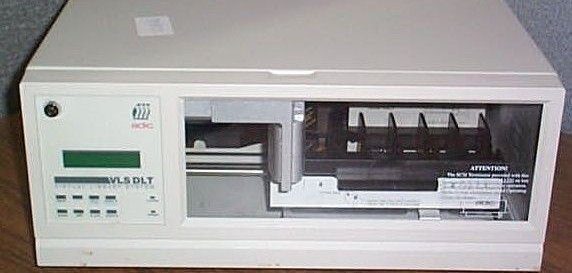
\includegraphics[scale=0.8]{pics/dlt-library.eps}
\end{center}
\vspace*{\fill}

\subsection{And now for something completely different...}
\begin{itemize}
	\item backup vs. restore
	\item backup devices and media
\end{itemize}
\vspace*{\fill}
\begin{center}
	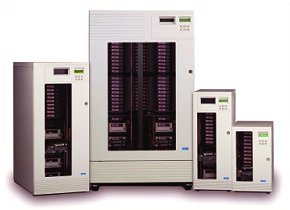
\includegraphics[scale=1.0]{pics/libraries.eps}
\end{center}
\vspace*{\fill}

\subsection{And now for something completely different...}
\begin{itemize}
	\item backup vs. restore
	\item backup devices and media
	\item filesystem considerations
\end{itemize}

\subsection{And now for something completely different...}
\begin{itemize}
	\item backup vs. restore
	\item backup devices and media
	\item filesystem considerations
	\item backup strategies
\end{itemize}

\subsection{And now for something completely different...}
\begin{itemize}
	\item backup vs. restore
	\item backup devices and media
	\item filesystem considerations
	\item backup strategies
	\item planning for disasters
\end{itemize}

\subsection{Backups and Restore Basics}
When do we need backups?

\subsection{Backups and Restore Basics}
When do we need backups?
\begin{itemize}
	\item disaster recovery: off-site storage of sensitive data
	\item long-term storage requirements
	\item recover from data loss
\end{itemize}

\subsection{Backups and Restore Basics}
When do we need backups?
\begin{itemize}
	\item disaster recovery: off-site storage of sensitive data
	\item long-term storage requirements
	\item recover from data loss due to
\end{itemize}
\vspace*{\fill}
\begin{center}
	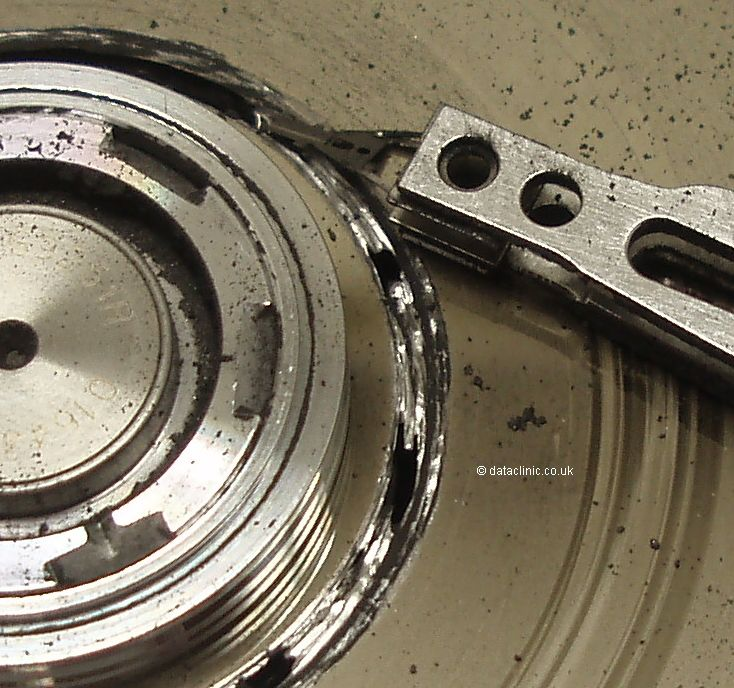
\includegraphics[scale=1.0]{pics/headcrash-closeup.eps}
\end{center}
\vspace*{\fill}

\subsection{Backups and Restore Basics}
When do we need backups?
\begin{itemize}
	\item disaster recovery: off-site storage of sensitive data
	\item long-term storage requirements
	\item recover from data loss due to
\end{itemize}
\vspace*{\fill}
\begin{center}
	
\includegraphics[scale=1.2]{pics/dumb-user.eps}
\end{center}
\vspace*{\fill}

\subsection{Backups and Restore Basics}
When do we need backups?
\begin{itemize}
	\item disaster recovery: off-site storage of sensitive data
	\item long-term storage requirements
	\item recover from data loss due to
\end{itemize}
\vspace*{\fill}
\begin{center}
	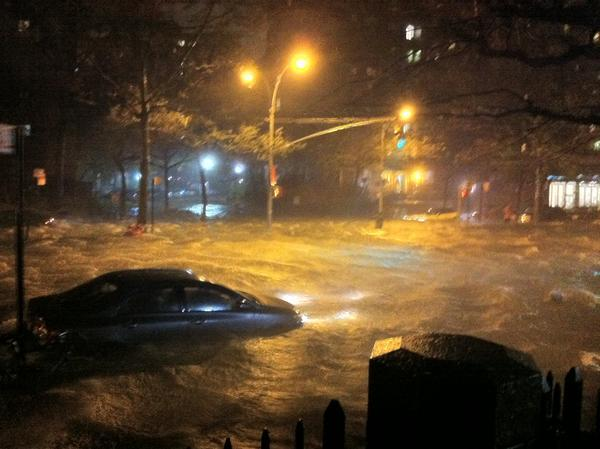
\includegraphics[scale=0.4]{pics/20th-and-C.eps}
\end{center}
\vspace*{\fill}

\subsection{Backups and Restore Basics}
When do we need backups?
\begin{itemize}
	\item disaster recovery: off-site storage of sensitive data
	\item long-term storage requirements
	\item recover from data loss due to
\end{itemize}
\vspace*{\fill}
\begin{center}
	
\includegraphics[scale=0.6]{pics/hacker.eps}
\end{center}
\vspace*{\fill}

\subsection{Backups and Restore Basics}
When do we need backups?
\begin{itemize}
	\item disaster recovery: off-site storage of sensitive data
	\item long-term storage requirements
	\item recover from data loss due to
\end{itemize}
\vspace*{\fill}
\begin{center}
	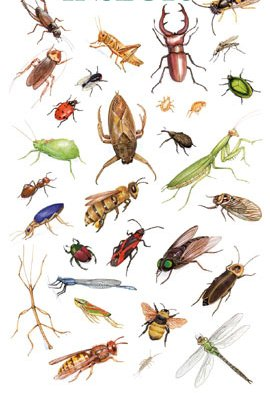
\includegraphics[scale=0.6]{pics/bugs.eps}
\end{center}
\vspace*{\fill}

\subsection{Backups and Restore Basics}
When do we need backups?
\begin{itemize}
	\item disaster recovery: off-site storage of sensitive data
	\item long-term storage requirements
	\item recover from data loss due to
		\begin{itemize}
			\item equipment failure
			\item bozotic users
			\item natural disaster
			\item security breach
			\item software bugs
		\end{itemize}
\end{itemize}

\subsection{Backups and Restore Basics}
When do we need backups?
\begin{itemize}
	\item disaster recovery: off-site storage of sensitive data
	\item long-term storage requirements
	\item recover from data loss due to
		\begin{itemize}
			\item equipment failure
			\item bozotic users
			\item natural disaster
			\item security breach
			\item software bugs
		\end{itemize}
\end{itemize}
\addvspace{.5in}
Think of your backups as {\em insurance}:  you invest and pay for it, hoping
you will never need it.


\subsection{Key Reasons for Restores}
Three key reasons for restores: {\em Accidental File Deletion}, {\em Disk
Failure} and {\em Archival}.
\\

1. Accidental File Deletion
\begin{itemize}
	\item ability to restore a file within a certain time frame
	\item restore time, including
		\begin{itemize}
			\item actual time spent restoring
			\item waiting until resources permit the restore
			\item staff availability
		\end{itemize}
	\item self-service restore
\end{itemize}

\subsection{Key Reasons for Restores}
2. Disk Failure
\begin{itemize}
	\item loss of entire file system
	\item leads to downtime
	\item RAID may help
	\item takes long time to restore
\end{itemize}
\addvspace{.5in}
3. Archival
\begin{itemize}
	\item {\em full} set of level 0 backups
	\item separate set from regular backups
	\item usually stored off-site
	\item store for long time
\end{itemize}

\subsection{Filesystem backup}
{\tt dump(8)} / {\tt restore(8)}
\begin{itemize}
	\item in use since \~{}1975
	\item full filesystem level backups
	\item direct interaction with tape devices
	\item integration with {\tt /etc/fstab}
	\item efficient incremental backups
\end{itemize}

\subsection{Filesystem backup}
\vspace*{\fill}
\begin{center}
	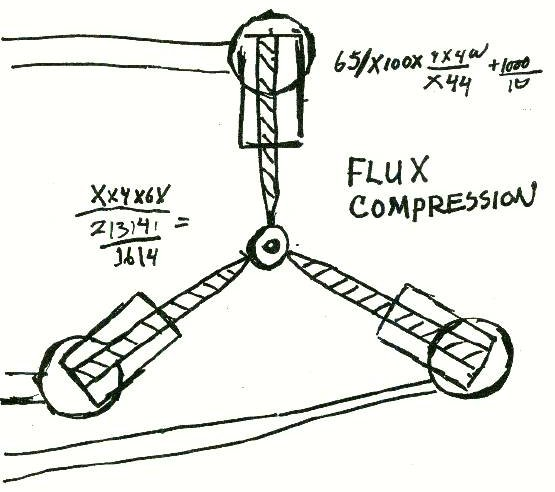
\includegraphics[scale=0.7]{pics/flux-capacitor.eps}
\end{center}
\vspace*{\fill}

\subsection{Filesystem backup}
\vspace*{\fill}
\begin{center}
	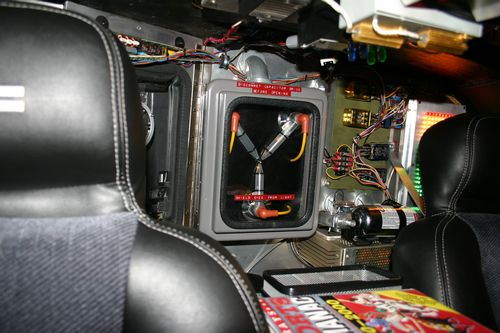
\includegraphics[scale=2.5]{pics/flux-capacitor2.eps}
\end{center}
\vspace*{\fill}

\subsection{Filesystem backup}
\vspace*{\fill}
\begin{center}
	
\includegraphics[scale=0.6]{pics/Time_Machine.eps}
\end{center}
\vspace*{\fill}


\subsection{Filesystem backup}
Example: Mac OS X ``Time Machine'':
\begin{itemize}
	\item automatically creates a full backup (equivalent of a "level 0 dump")
		to separate device or NAS, recording (specifically) last-modified date
		of all directories
	\item every hour, creates a full copy via {\em hardlinks} (hence no
		additional disk space consumed) for files that have not changed,
		new copy of files that have changed
		\item changed files are determined by inspecting last-modified date of
			directories (cheaper than doing comparison of all files'
			last-modified date or data)
	\item saves hourly backups for 24 hours, daily backups for
		the past month, and weekly backups for everything older than a month.
\end{itemize}

\subsection{Filesystem backup}
Example: WAFL (Write Anywhere File Layout)
\begin{itemize}
	\item used by NetApp's ``Data ONTAP'' OS
	\item a snapshot is a read-only copy of a file system (cheap and near
		instantaneous, due to CoW)
	\item uses regular snapshots (``consistency points'', every 10 seconds)
		to allow for speedy recovery from crashes
\end{itemize}
\vspace*{\fill}
\begin{center}
	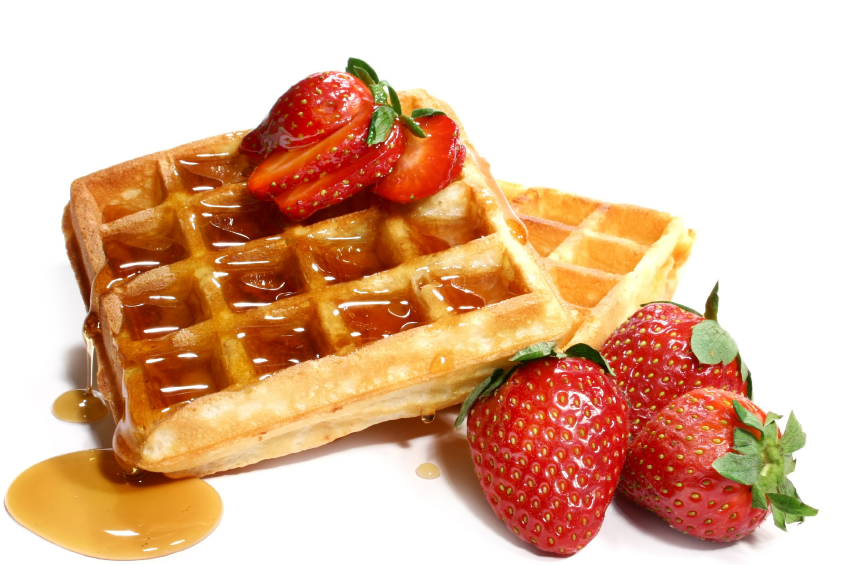
\includegraphics[scale=0.75]{pics/waffles.eps}
\end{center}
\vspace*{\fill}


\subsection{Filesystem backup}
Example: WAFL (Write Anywhere File Layout)
\vspace*{\fill}
\begin{center}
	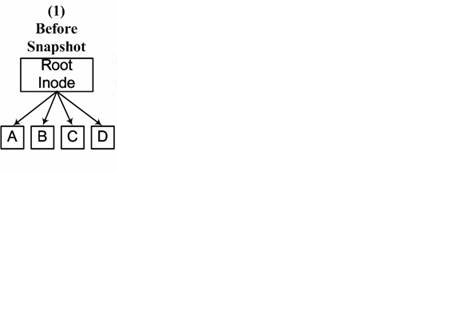
\includegraphics[scale=1.0]{pics/wafl0.eps}
\end{center}
\vspace*{\fill}


\subsection{Filesystem backup}
Example: WAFL (Write Anywhere File Layout)
\vspace*{\fill}
\begin{center}
	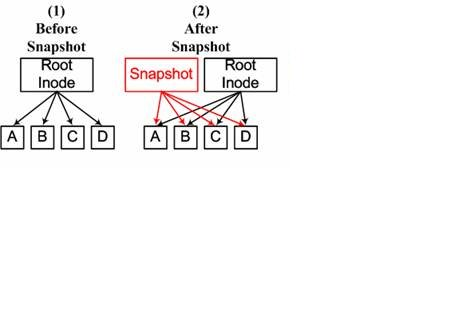
\includegraphics[scale=1.0]{pics/wafl1.eps}
\end{center}
\vspace*{\fill}


\subsection{Filesystem backup}
Example: WAFL (Write Anywhere File Layout)
\vspace*{\fill}
\begin{center}
	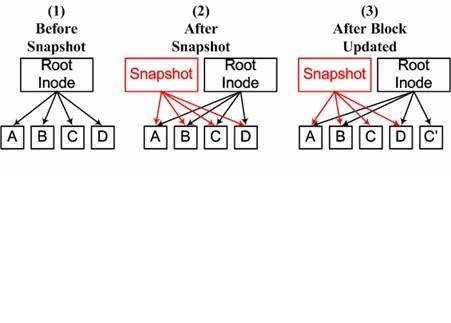
\includegraphics[scale=1.0]{pics/wafl2.eps}
\end{center}
\vspace*{\fill}


\subsection{Filesystem backup}
Example: WAFL (Write Anywhere File Layout)
\vspace*{\fill}
\begin{center}
	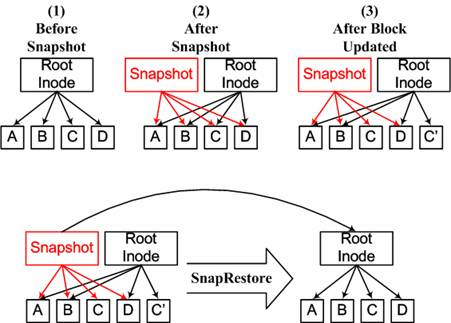
\includegraphics[scale=1.0]{pics/wafl.eps}
\end{center}
\vspace*{\fill}


\subsection{Filesystem backup}
Example: ZFS snapshots
\begin{itemize}
	\item ZFS uses a copy-on-write transactional object model (new data does
		not overwrite existing data, instead modifications are written to a
		new location with existing data being referenced), similar to WAFL
	\item a snapshot is a read-only copy of a file system (cheap and near
		instantaneous, due to CoW)
	\item initially consumes no additional disk space; the writable filesystem
		is made available as a ``clone''
	\item conceptually provides a branched view of the filesystem; normally
		only the ``active'' filesystem is writable
\end{itemize}

\subsection{ZFS Snapshots}
\smallish
\begin{verbatim}
$ pwd
/home/jschauma
$ ls -l .z*
ls: cannot access .z*: No such file or directory
$
\end{verbatim}
\Normalsize

\subsection{ZFS Snapshots}
\smallish
\begin{verbatim}
$ pwd
/home/jschauma
$ ls -l .z*
ls: cannot access .z*: No such file or directory
$ ls -lid .zfs
1 dr-xr-xr-x 3 root root 3 Jan 10  2013 .zfs
$
\end{verbatim}
\Normalsize

\subsection{ZFS Snapshots}
\smallish
\begin{verbatim}
$ pwd
/home/jschauma
$ ls -l .z*
ls: cannot access .z*: No such file or directory
$ ls -lid .zfs
1 dr-xr-xr-x 3 root root 3 Jan 10  2013 .zfs
$ ls -lai .zfs/snapshot
total 13
2 dr-xr-xr-x  4 root     root       4 Feb 28 21:00 .
1 dr-xr-xr-x  3 root     root       3 Jan 10  2013 ..
4 drwx--x--x 37 jschauma professor 88 Feb 24 22:32 amanda-_export_home_jschauma-0
4 drwx--x--x 37 jschauma professor 88 Feb 26 11:47 amanda-_export_home_jschauma-1
$
\end{verbatim}
\Normalsize

\subsection{ZFS Snapshots}
\smallish
\begin{verbatim}
$ pwd
/home/jschauma
$ ls -l .z*
ls: cannot access .z*: No such file or directory
$ ls -lid .zfs
1 dr-xr-xr-x 3 root root 3 Jan 10  2013 .zfs
$ ls -lai .zfs/snapshot
total 13
2 dr-xr-xr-x  4 root     root       4 Feb 28 21:00 .
1 dr-xr-xr-x  3 root     root       3 Jan 10  2013 ..
4 drwx--x--x 37 jschauma professor 88 Feb 24 22:32 amanda-_export_home_jschauma-0
4 drwx--x--x 37 jschauma professor 88 Feb 26 11:47 amanda-_export_home_jschauma-1
$ cd .zfs/snapshot
$ echo foo > amanda-_export_home_jschauma-0/oink
-ksh: amanda-_export_home_jschauma-0/oink: cannot create [Read-only file system]
$ ls -laid . /
2 dr-xr-xr-x  4 root root    4 Feb 28 21:00 .
2 drwxr-xr-x 26 root root 4096 Jan 27 11:44 /
\end{verbatim}
\Normalsize

\subsection{ZFS Snapshots}
\smallish
\begin{verbatim}
$ pwd
/home/jschauma/.zfs/snapshot
$ ls -lai amanda-_export_home_jschauma-0 >/tmp/a
$ ls -lai amanda-_export_home_jschauma-1 >/tmp/b
$ diff -bu /tmp/[ab]
--- /tmp/a	2014-03-01 22:55:49.000000000 -0500
+++ /tmp/b	2014-03-01 22:55:59.000000000 -0500
@@ -35,7 +35,7 @@
 57723 drwx------  3 jschauma professor         6 Dec 31 15:08 .subversion
 49431 -rw-------  1 jschauma professor         6 Dec 22 12:25 .sws.pid
    20 drwx------  2 jschauma professor         3 Jan 26 10:30 .vim
-61768 -rw-------  1 jschauma professor     14538 Feb 24 22:32 .viminfo
+61775 -rw-------  1 jschauma professor     14557 Feb 26 09:23 .viminfo
   173 -rw-------  1 jschauma professor      4355 Sep 17  2012 .vimrc
 45744 -rw-r--r--  1 jschauma professor         0 Jul 28  2013 .xsession-errors
    21 drwxr-xr-x  3 jschauma professor         6 Apr  4  2010 CS615A
$
\end{verbatim}
\Normalsize

\subsection{HW \#4}
Data backup to the cloud \\
\verb+http://www.cs.stevens.edu/~jschauma/615/s14-hw4.html+
\\
\verb+http://www.cs.stevens.edu/~jschauma/615/ec2-backup.txt+

\subsection{Reading}
\begin{itemize}
	\item \verb+https://en.wikipedia.org/wiki/Unix_philosophy+
	\item \verb+http://is.gd/jDDGpW+
	\item \verb+http://is.gd/bXG9of+
\end{itemize}

\subsection{Reading}
Hurricane Sandy
\begin{itemize}
	\item \verb+http://is.gd/aaxzvI+
	\item \verb+http://is.gd/Y75pEA+
	\item \verb+http://is.gd/32Az7y+
	\item \verb+http://is.gd/FhAuFZ+
\end{itemize}

\subsection{Reading}
Manual Pages:
\begin{itemize}
	\item \verb+dump(8)+ and \verb+restore(8)+
\end{itemize}
Filesystem snapshots:
\begin{itemize}
	\item \verb+https://en.wikipedia.org/wiki/Snapshot_(computer_storage)+
	\item \verb+https://en.wikipedia.org/wiki/Time_Machine_(Apple_software)+
	\item \verb+http://comet.lehman.cuny.edu/jung/cmp426697/WAFL.pdf+
	\item \verb+http://www.cs.tau.ac.il/~ohadrode/slides/WAFL.pdf+
\end{itemize}
\vspace{.5in}
Book: \verb+http://www.oreilly.com/catalog/unixbr/+

\end{document}
